
\section{Simulations}


\begin{table}[H]
    \begin{center}
        \caption{Size of the test calculated for different sample sizes ($T = 250, 350, 500, 1000$) and confident levels ($\alpha = 0.01, 0.05, 0.10$)}
        \label{tab:size_nw}
        \centering
        % latex table generated in R 3.4.3 by xtable 1.8-2 package
% 
\begin{tabular}{rrrr}
  \hline
 & 0.01 & 0.05 & 0.1 \\ 
  \hline
250 & 0.02 & 0.04 & 0.10 \\ 
  350 & 0.01 & 0.05 & 0.10 \\ 
  500 & 0.01 & 0.05 & 0.09 \\ 
   \hline
\end{tabular}

    \end{center}
\end{table}

\begin{table}[H]
    \begin{center}
        \caption{Power of the test calculated for different sample sizes ($T = 250, 350, 500, 1000$) and confident levels ($\alpha = 0.01, 0.05, 0.10$) for $a = 0.25$}
        \label{tab:power_025_nw}
        \centering
        % latex table generated in R 3.4.3 by xtable 1.8-2 package
% 
\begin{tabular}{rrrr}
  \hline
 & 0.01 & 0.05 & 0.1 \\ 
  \hline
250 & 0.04 & 0.16 & 0.26 \\ 
  350 & 0.08 & 0.21 & 0.36 \\ 
  500 & 0.14 & 0.31 & 0.41 \\ 
   \hline
\end{tabular}

    \end{center}
\end{table}

\begin{table}[H]
    \begin{center}
        \caption{Power of the test calculated for different sample sizes ($T = 250, 350, 500, 1000$) and confident levels ($\alpha = 0.01, 0.05, 0.10$) for $a = 0.50$}
        \label{tab:power_050_nw}
        \centering
        % latex table generated in R 3.4.3 by xtable 1.8-2 package
% 
\begin{tabular}{rrrr}
  \hline
 & 0.01 & 0.05 & 0.1 \\ 
  \hline
250 & 0.36 & 0.61 & 0.73 \\ 
  350 & 0.60 & 0.79 & 0.89 \\ 
  500 & 0.81 & 0.94 & 0.97 \\ 
   \hline
\end{tabular}

    \end{center}
\end{table}

\begin{table}[H]
    \begin{center}
        \caption{Power of the test calculated for different sample sizes ($T = 250, 350, 500, 1000$) and confident levels ($\alpha = 0.01, 0.05, 0.10$) for $a = 0.65$}
        \label{tab:power_065_nw}
        \centering
        % latex table generated in R 3.4.3 by xtable 1.8-2 package
% 
\begin{tabular}{rrrr}
  \hline
 & 0.01 & 0.05 & 0.1 \\ 
  \hline
250 & 0.70 & 0.85 & 0.91 \\ 
  350 & 0.90 & 0.97 & 0.98 \\ 
  500 & 0.99 & 1.00 & 1.00 \\ 
   \hline
\end{tabular}

    \end{center}
\end{table}

\begin{table}[H]
    \begin{center}
        \caption{Power of the test calculated for different sample sizes ($T = 250, 350, 500, 1000$) and confident levels ($\alpha = 0.01, 0.05, 0.10$) for $a = 0.75$}
        \label{tab:power_075_nw}
        \centering
        % latex table generated in R 3.4.3 by xtable 1.8-2 package
% 
\begin{tabular}{rrrr}
  \hline
 & 0.01 & 0.05 & 0.1 \\ 
  \hline
250 & 0.86 & 0.95 & 0.98 \\ 
  350 & 0.98 & 0.99 & 1.00 \\ 
  500 & 1.00 & 1.00 & 1.00 \\ 
   \hline
\end{tabular}

    \end{center}
\end{table}

\begin{table}[H]
    \begin{center}
        \caption{Power of the test calculated for different sample sizes ($T = 250, 350, 500, 1000$) and confident levels ($\alpha = 0.01, 0.05, 0.10$) for $a = 1.0$}
        \label{tab:power_100_nw}
        \centering
        % latex table generated in R 3.4.3 by xtable 1.8-2 package
% 
\begin{tabular}{rrrr}
  \hline
 & 0.01 & 0.05 & 0.1 \\ 
  \hline
250 & 0.99 & 1.00 & 1.00 \\ 
  350 & 1.00 & 1.00 & 1.00 \\ 
  500 & 1.00 & 1.00 & 1.00 \\ 
   \hline
\end{tabular}

    \end{center}
\end{table}


\begin{table}[H]
    \begin{center}
        \caption{Size of the test calculated for different sample sizes ($T = 250, 350, 500, 1000$) and confident levels ($\alpha = 0.01, 0.05, 0.10$)}
        \label{tab:size_ll}
        \centering
        % latex table generated in R 3.4.3 by xtable 1.8-2 package
% 
\begin{tabular}{rrrr}
  \hline
 & 0.01 & 0.05 & 0.1 \\ 
  \hline
250 & 0.01 & 0.05 & 0.11 \\ 
  350 & 0.01 & 0.05 & 0.09 \\ 
  500 & 0.01 & 0.05 & 0.09 \\ 
   \hline
\end{tabular}

    \end{center}
\end{table}

\begin{table}[H]
    \begin{center}
        \caption{Power of the test calculated for different sample sizes ($T = 250, 350, 500, 1000$) and confident levels ($\alpha = 0.01, 0.05, 0.10$) for $a = 0.25$}
        \label{tab:power_025_ll}
        \centering
        % latex table generated in R 3.4.3 by xtable 1.8-2 package
% 
\begin{tabular}{rrrr}
  \hline
 & 0.01 & 0.05 & 0.1 \\ 
  \hline
250 & 0.12 & 0.26 & 0.36 \\ 
  350 & 0.13 & 0.32 & 0.46 \\ 
  500 & 0.24 & 0.47 & 0.59 \\ 
   \hline
\end{tabular}

    \end{center}
\end{table}

\begin{table}[H]
    \begin{center}
        \caption{Power of the test calculated for different sample sizes ($T = 250, 350, 500, 1000$) and confident levels ($\alpha = 0.01, 0.05, 0.10$) for $a = 0.50$}
        \label{tab:power_050_ll}
        \centering
        % latex table generated in R 3.4.3 by xtable 1.8-2 package
% 
\begin{tabular}{rrrr}
  \hline
 & 0.01 & 0.05 & 0.1 \\ 
  \hline
250 & 0.65 & 0.82 & 0.89 \\ 
  350 & 0.79 & 0.94 & 0.96 \\ 
  500 & 0.94 & 0.99 & 1.00 \\ 
   \hline
\end{tabular}

    \end{center}
\end{table}

\begin{table}[H]
    \begin{center}
        \caption{Power of the test calculated for different sample sizes ($T = 250, 350, 500, 1000$) and confident levels ($\alpha = 0.01, 0.05, 0.10$) for $a = 0.65$}
        \label{tab:power_065_ll}
        \centering
        % latex table generated in R 3.4.3 by xtable 1.8-2 package
% 
\begin{tabular}{rrrr}
  \hline
 & 0.01 & 0.05 & 0.1 \\ 
  \hline
250 & 0.92 & 0.98 & 0.98 \\ 
  350 & 0.98 & 1.00 & 1.00 \\ 
  500 & 1.00 & 1.00 & 1.00 \\ 
   \hline
\end{tabular}

    \end{center}
\end{table}

\begin{table}[H]
    \begin{center}
        \caption{Power of the test calculated for different sample sizes ($T = 250, 350, 500, 1000$) and confident levels ($\alpha = 0.01, 0.05, 0.10$) for $a = 0.75$}
        \label{tab:power_075_ll}
        \centering
        % latex table generated in R 3.4.3 by xtable 1.8-2 package
% 
\begin{tabular}{rrrr}
  \hline
 & 0.01 & 0.05 & 0.1 \\ 
  \hline
250 & 0.99 & 0.99 & 1.00 \\ 
  350 & 1.00 & 1.00 & 1.00 \\ 
  500 & 1.00 & 1.00 & 1.00 \\ 
   \hline
\end{tabular}

    \end{center}
\end{table}

\begin{table}[H]
    \begin{center}
        \caption{Power of the test calculated for different sample sizes ($T = 250, 350, 500, 1000$) and confident levels ($\alpha = 0.01, 0.05, 0.10$) for $a = 1.0$}
        \label{tab:power_100_ll}
        \centering
        % latex table generated in R 3.4.3 by xtable 1.8-2 package
% 
\begin{tabular}{rrrr}
  \hline
 & 0.01 & 0.05 & 0.1 \\ 
  \hline
250 & 1.00 & 1.00 & 1.00 \\ 
  350 & 1.00 & 1.00 & 1.00 \\ 
  500 & 1.00 & 1.00 & 1.00 \\ 
   \hline
\end{tabular}

    \end{center}
\end{table}



\newpage
\section{Data analysis}


\begin{figure}[ht!]
\centering
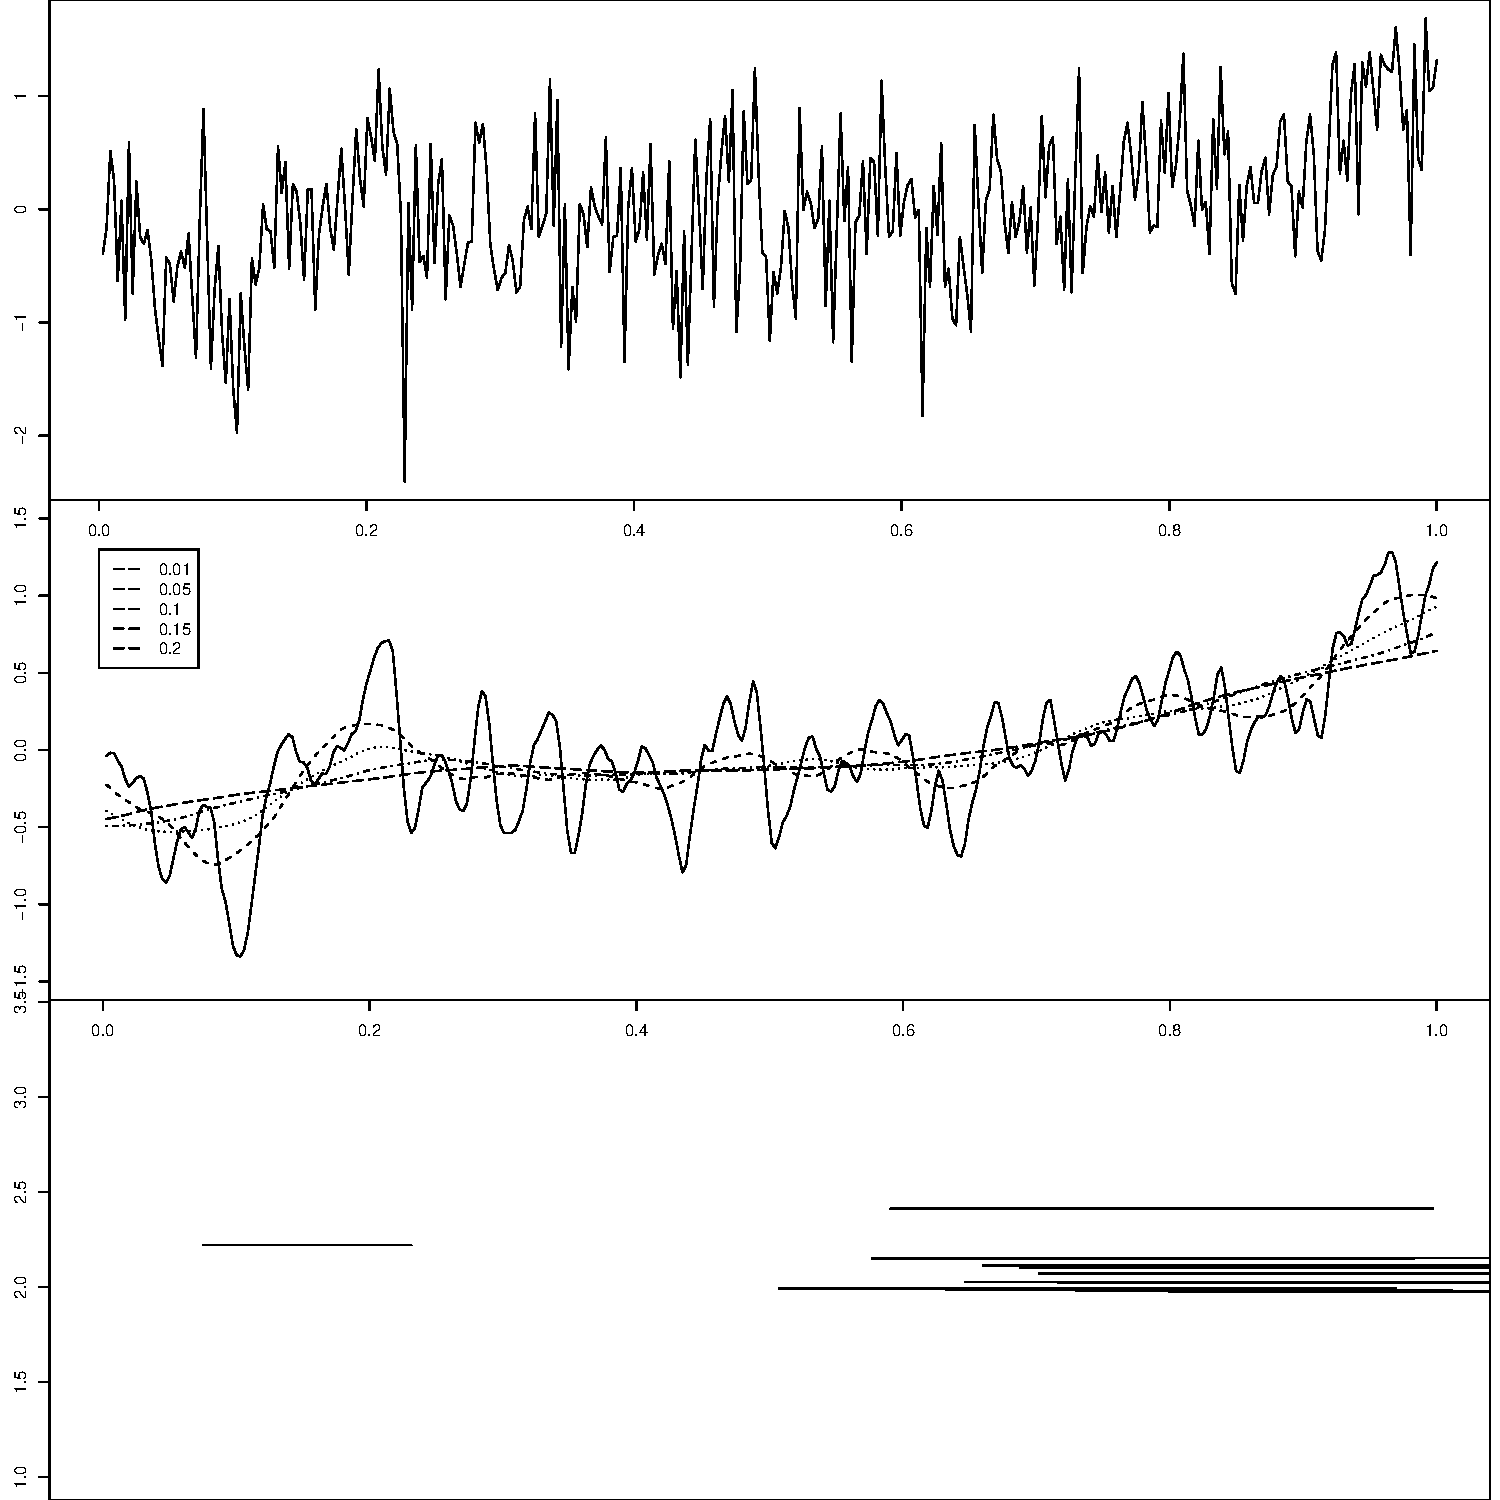
\includepdf[pages=-,pagecommand={},width=\textwidth]{Coding/Output/threegraphics.pdf}
\caption{Yearly temperature data for England\label{yearly_data}}
\end{figure}

